Окно настроек содержит элементы интерфейса, которые позволяют правильно настроить программу для
работы с устройством считывателя. Окно разделено на две части соответствующими вкладками: <<Файлы/Метки/События>> и
<<Подключенные устройства>>.

\subsection{Вкладка: Файлы/Метки/События}

Активировав вкладку
<<Файлы/Метки/События>> (рис. \ref{i:stag}), пользователь получает возможность изменять настройки приложения. Верхние две строки вкладки
позволяют открыть или создать новые файлы журнала и настроек. 

\begin{figure}[h]
    \center{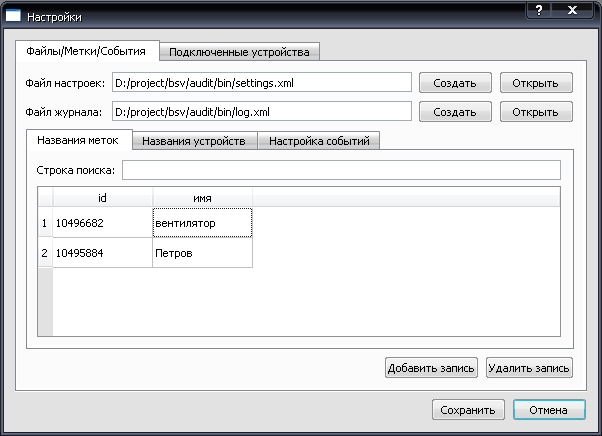
\includegraphics[scale=0.5]{img/settings_tag.png}}
    \caption{Окно настроек файлов/меток/событий}
    \label{i:stag}
\end{figure}

При открытии файла настроек, вся информация
из файла о настройках загружается в приложение и отображается в соответствующих местах интерфейса: информация о синонимах меток
ниже во вкладке <<Названия меток>>, информация о 
настройках реакций на события во вкладке <<Настройка событий>>. Программа также загружает данные о 
настройках устройств, ранее сконфигурированных в программе.

Для сохранения новых настроек приложения, необходимо нажать на кнопку <<Сохранить>> при активной вкладке
<<Файлы/Метки/События>>. При нажатии на кнопку <<Отмена>>, окно настроек закрывается.

При открытии файла журнала, информация о сохраненных в нем событиях отображается в окне монитора в виде таблицы.
Если файл хранит много данных, то показывается окно статуса процесса загрузки, где в процентах отображается
степень готовности операции чтения файла журнала.  

\subsubsection{Вкладка: Названия меток}

Для упрощения задач учета и контроля меток, в программе можно давать числовым идентификаторам меток
символьные имена. 

Вкладка <<Названия меток>> позволяет просматривать и редактировать информацию о синонимах меток. 
Редактирование осуществляется прямо в таблице, отображаемой во вкладке. Для удаления, необходимо выделить ненужную 
запись и нажать кнопку <<Удалить запись>>. Добавление новой записи производится посредством нажатия на
кнопку <<Добавить запись>>. Также в окне есть строка поиска, куда можно вводить ключевые слова, по которым
будет осуществлен поиск по таблице синонимов меток. Результаты поиска отобразятся сразу же в этой же таблице.

Чтобы сохранить изменения в файле настроек, нужно нажать кнопку <<Сохранить>>.

\subsubsection{Вкладка: Настройка событий}

Для выделения отдельных событий из всех случившихся, в программе можно настраивать определенную реакцию
на предполагаемое событие (рис. \ref{i:sevent}). 

Предусмотрено два вида событий: обнаружен новый таг либо таг потерян. На эти события возможно отреагировать двумя способами.
Либо выделить цветом событие в окне монитора, либо выдать сообщение о происшествии данного события.
В случае показа сообщения, программа регистрирует в файле журнала факт реакции оператора на него. Фиксируется закрытие
оператором окна с оповещением о событии.

Настройка реакций на события происходит путем редактирования таблицы в данной вкладке. Ячейки с именем устройства, именем метки, 
номером канала, событием и реакцией
изменяются посредством выпадающих списков. Причем при выборе реакции <<выделить цветом>>, открывается диалоговое окно с цветовой палитрой, где
пользователь может выбрать необходимый цвет подсветки события. 

В выпадающем списке выбора имени устройства отображаются только подключенные и обнаруженные программой устройства. Имя для метки можно выбрать из
выпадающего списка, который содержит синонимы, присвоенные меткам на вкладке "Файлы/Метки/События".
Ячейка с именем события изменяется как текстовое поле. 

Для удаления, необходимо выделить ненужную 
запись и нажать кнопку <<Удалить запись>>. Добавление новой записи производится посредством нажатия на
кнопку <<Добавить запись>>. 
Чтобы сохранить изменения в файле настроек, нужно нажать кнопку <<Сохранить>>.

\begin{figure}[h]
    \center{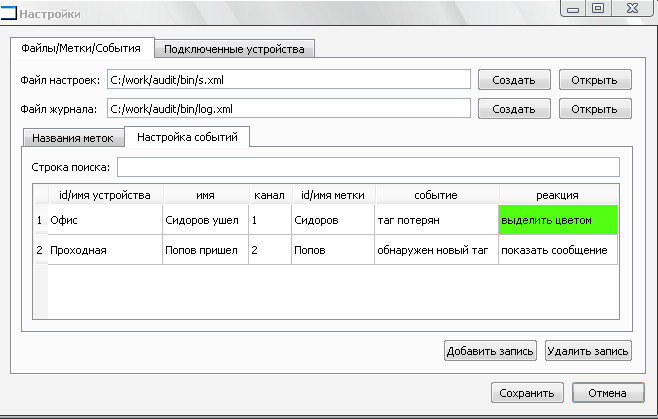
\includegraphics[scale=0.5]{img/settings_event.png}}
    \caption{Окно настроек событий}
    \label{i:sevent}
\end{figure}

\subsection{Вкладка: Подключенные устройства}

Элементы интерфейса на данной вкладке позволяют настраивать подключенные к компьютеру считыватели (рис. \ref{i:sdev}).
При нажатии на кнопку <<Найти устройства>>, программа отображает информацию о параллельно подключенных к USB портам устройствах в
виде списка в верхней части окна. 

\begin{figure}[h]
    \center{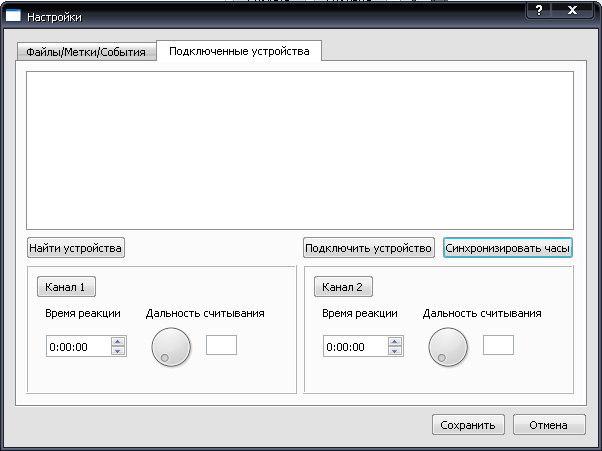
\includegraphics[scale=0.5]{img/settings_dev.png}}
    \caption{Окно настроек и подключения устройств}
    \label{i:sdev}
\end{figure}

При нажатии на кнопку <<Синхронизировать часы>>, обновляется время внутренних часов для всех обнаруженных считывателей.
Чтобы поправить настройки для отдельного устройства, необходимо выбрать его щелчком левой клавиши мышки в списке.
После этого информация о текущих его настройках отобразится в нижней части окна. 
Подключение и отключение каналов происходит по нажатию на кнопках <<Канал 1>>, <<Канал 2>>.
Если канал включен, то соответствующая кнопка отображается в нажатом состоянии.

Для настройки расположенных последовательно на одной шине устройств необходимо добавить иформацию о них в таблицу. 
Для этого нужно дважды щелкнуть левой кнопкой мыши на строке с подключенным корневым устройством. Добавленному устройству
можно назначить адрес и имя. Имя устройства будет отображаться в таблице монитора при регистрации транзакций от данного считывателя.

Щелкнув правой кнопкой мыши на строке со считывателем, откроется контекстное меню дополнительных настроек (рис. \ref{i:scontext}). Это меню позваляет назначить новый
адрес устройству (при этом на шине должен находиться только один считыватель), получить (обновить) настройки или удалить устройство. 

\begin{figure}[h]
    \center{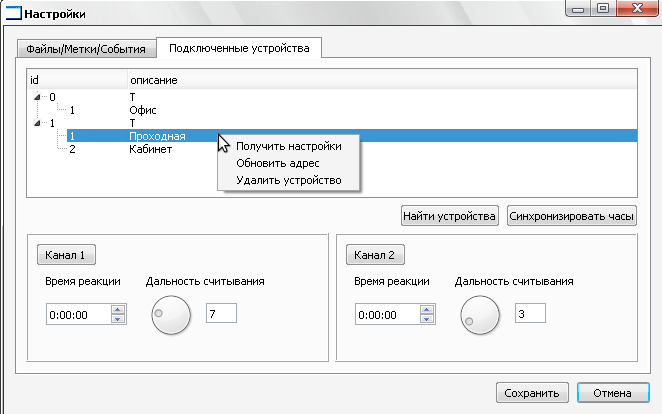
\includegraphics[scale=0.5]{img/settings_context.png}}
    \caption{Контекстное меню в окне настроек устройств}
    \label{i:scontext}
\end{figure}

Чтобы изменить адрес, необходимо щелкнуть правой кнопкой мыши на строке со считывателем и выбрать в выпадающем меню <<Обновить адрес>>. Откроется 
диалоговое окно смены адреса. Допустимый диапазон адресов: 0 - 255. Адреса 0, 3, 255 зарезервированы для служебных целей.

Обновление настроек необходимо для загрузки в программу текущих настроек устройства 
(актуально когда подключается новый считыватель, настройки которого пока неизвестны программе).

После обнаружения устройств, программа начнет считывать данные из их журналов транзакций и 
отображать их в окне монитора. Подключение и отключение каналов происходит по нажатию на кнопках <<Канал 1>>, <<Канал 2>>.
Если канал включен, то соответствующая кнопка отображается в нажатом состоянии.

Настройка считывателя в соответствии с заданными параметрами производится после нажатия на кнопку <<Сохранить>>.
Если есть необходимость внести эти настройки в файл настроек, то нужно переключиться на вкладку <<Файлы/Метки/События>>
 и нажать на кнопку <<Сохранить>>.

